
% Lecture Template for ME3023 -  Measurements in Mechanical Systems - Tennessee Technological University
% Spring 2020 - Summer 2020 - Fall 2020 - Spring 2021 - Summer 2021
% Tristan Hill, May 07, 2020 - June 12, 2020 - July 08, 2020 - Novemeber 02, 2020 - March 28, 2021 - May 25, 2021
% Module Name: - Introduction
% Topic 3 - Experimental Test Plan

\documentclass[fleqn]{beamer} % for presentation (has nav buttons at bottom)

%\usepackage{/home/thill/Documents/lectures/measurements_lectures/measurements_lectures}
\usepackage{/home/tntech.edu/thill/courses/measurements/lectures/measurements_lectures}


\author{ME3023 - Measurements in Mechanical Systems} % original formatting from Mike Renfro, September 21, 2004

\newcommand{\TNUM}{3\hspace{2mm}} % Topic number 
\newcommand{\moduletitle}{Introduction}
\newcommand{\topictitle}{Experimental Test Plan}

\newcommand{\sectiontitleI}{Parameter Design Plan}
\newcommand{\sectiontitleII}{System and Tolerance Design Plan}
\newcommand{\sectiontitleIII}{Data Reduction Design Plan}
\newcommand{\sectiontitleIV}{Experimental Design Strategies }
\newcommand{\sectiontitleV}{Small Group Activity}


% custom box
\newsavebox{\mybox}

\title{Lecture Module - \moduletitle}

\date{Mechanical Engineering\vspc Tennessee Technological University}


\begin{document}
	
\lstset{language=MATLAB,basicstyle=\ttfamily\small,showstringspaces=false}
	
\frame{\titlepage \center\begin{framed}\Large \textbf{Topic \TNUM - \topictitle}\end{framed} \vspace{5mm}}

% Section 0: Outline
\begin{frame}

\large \textbf{Topic \TNUM - \topictitle} \vspace{3mm}\\

\begin{itemize}

	\item \hyperlink{sectionI}{\sectiontitleI} \vspc % Section I
	\item \hyperlink{sectionII}{\sectiontitleII} \vspc % Section II
	\item \hyperlink{sectionIII}{\sectiontitleIII} \vspc %Section III
	\item \hyperlink{sectionIV}{\sectiontitleIV} \vspc %Section IV
	\item \hyperlink{sectionIV}{\sectiontitleV} \vspc %Section V

\end{itemize}

\end{frame}

% Section 1
\section{\sectiontitleI}

\begin{frame}[label=sectionI]
\frametitle{\sectiontitleI}

{\BL Parameter Design Plan}: Determine the test objective and identify the process variables and
parameters and a means for their control. \vspc
\underline{Ask}: \begin{itemize}
	\item 
	\item 
	\item 
\end{itemize} 

{\tiny Text: Theory and Design of Mech. Meas.}
\end{frame}

% Section 2
\section{\sectiontitleII}

\begin{frame}[label=sectionII]
\frametitle{\sectiontitleII}


{\PR System and Tolerance Design Plan}: Select a measurement technique, equipment, and
test procedure based on some preconceived tolerance limits for error. \vspc
\underline{Ask}:
\begin{itemize}
	\item 
	\item 
\end{itemize} 

{\tiny Text: Theory and Design of Mech. Meas.}
\end{frame}

% Section 3
\section{\sectiontitleIII}

\begin{frame}[label=sectionIII]
\frametitle{\sectiontitleIII}

{\GR Data Reduction Design Plan}: Plan how to analyze, present, and use the anticipated data.\vspc
\underline{Ask}:
\begin{itemize}
	\item 
	\item 
	\item 
	\item
\end{itemize} 

{\tiny Text: Theory and Design of Mech. Meas.}
\end{frame}

% Section 4
\section{\sectiontitleIV}

\begin{frame}[label=sectionIV]
\frametitle{\sectiontitleIV}


\begin{itemize}
	\item {\BL Randomized} Tests \vspccc% Section 1
	\item {\GR Repetition} and {\PR Replication}. \vspccc% Section 1
	\item {\BR Concomitant} Methods \vspccc
\end{itemize}

\end{frame}





	\begin{frame}[label=sectionV]
		\frametitle{\sectiontitleV}
			\tiny
		
		Group Activity: Find a group of 2-3 students. Complete the activity and submit your work on ilearn {\it as an indiviual}. You may submit the same or similar answers as your group members.	

	        \begin{multicols}{2}
		
		    \textbf{Experimental Test Plan: Fuel/Energy Economy} \\
		    %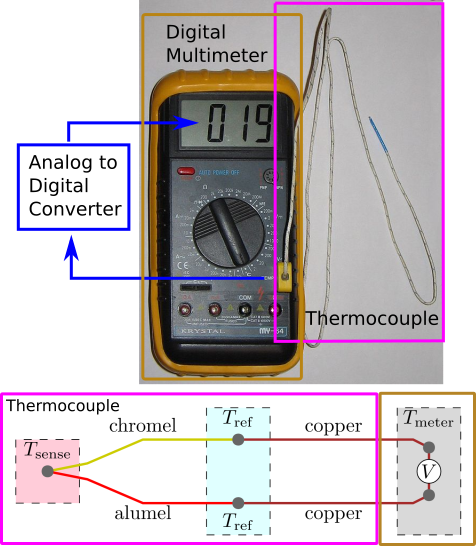
\includegraphics[scale=0.35]{thermocouple_atd.png} \vspc

		    \begin{enumerate}

		    	\item Develop an experimental test plan for determining the milage cost of your vehicle (choose any vehicle) in dollars per mile. Write a short desciption of the system. (paragraph or bulleted list)
			    
			    \vspace{5mm}

			    \item Identify the following variables for your plan.
				
			    \begin{multicols}{2}
				\begin{itemize}\tiny
					\item Measured Variable: 
					\item Independent Variable(s): 
					\item Dependent Variable(s): 
					\item Controlled Variable(s): 
					\item Extraneous Variable(s):
				\end{itemize}
				\end{multicols}	

				\vspace{12mm}

				\item Do you expect the results of the study to represent the true milage of the vehicle? How could you validate (or check) the results?


				\item What could you do to improve the results of the proposed study?

			\end{enumerate}
			
			\end{multicols}	

			%{\tiny Image, More Info: \href{https://en.wikipedia.org/wiki/Thermocouple}{Wikipedia} }\hspace{40mm} 

	\end{frame}


\end{document}